% Intended LaTeX compiler: pdflatex
\documentclass[10pt,a4paper,UTF8]{article}
\usepackage{zclorg}
\usepackage{tikztheorem}
\author{zcl.space}
\date{}
\title{Convergence of Sequence}
\hypersetup{
 pdfauthor={zcl.space},
 pdftitle={Convergence of Sequence},
 pdfkeywords={PMA},
 pdfsubject={},
 pdfcreator={Emacs 25.0.50.1 (Org mode 9.1.2)},
 pdflang={English}}
\begin{document}

\maketitle
\tableofcontents
\titlepic{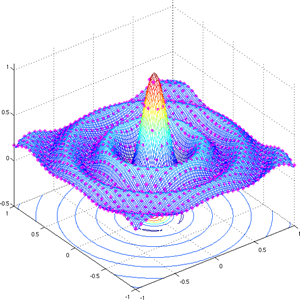
\includegraphics[scale=0.25]{../../img/sinc.PNG}}
 A \textbf{sequence} is a function defined on a subset of the
integers. (Usually this subset is the set
\(\mathbb{Z}^+:=\{n\in\mathbb{Z}:n > 0\}\) of positive integers or the set \(\mathbb{N}:=\{n\in\mathbb{Z}:n\ge 0\}\) of nonnegative inregers. )

It is customary to denote the value of a sequence at an integer \(n\)
with a subscript rather than with parentheses and to denote a sequence
with a notation like \((p_n)_n\) or \((p_n)_{n\in\mathbb{Z}^+}\).


\begin{definition}
The sequence \((p_n)_n\) of points of \(\mathbb{R}^m\) is said
to \textbf{converge} to the point \(p\in\mathbb{R}^m\)
iff
\begin{equation*}
   \lim_{n\to\infty} p_n=p
\end{equation*}
This is sometimes abbreviated as  \(p_n\to p\) as \(n\to\infty\).
We say a sequence \textbf{converges} or is \textbf{convergent}
iff it converges to \(p\) for some \(p\in\mathbb{R}^m\).
A sequence is said to \textbf{diverge}  when it does not converge.
(A sequence in \(\mathbb{R}\) whose limit is infinite is also said to diverge.)
\end{definition}

\begin{remark}
 Using the lingo introduced in\textasciitilde{}\ref{extended_reals} this may be stated as
$$
   \lim_{n\to\infty} p_n=p
$$
iff for every \(\epsilon > 0\)   there exists \(N=N(\epsilon) > 0\) such that
\(n\ge N\implies |p_n-p| < \epsilon\).
\end{remark}

\begin{theorem}
Assume that \((a_n)_n\) and \((b_n)_n\) are convergent sequences of real numbers:
\begin{equation*}
\lim_{n\to\infty} a_n = a, \qquad \lim_{n\to\infty} b_n=b.
\end{equation*}
Then
\begin{equation*}
\lim_{n\to\infty} a_n+b_n = a+b, \qquad \lim_{n\to\infty} a_nb_n = ab.
\end{equation*}
Moreover, if \(b\ne 0\) then \(b_n\ne 0\) for sufficiently large \(n\) and
\begin{equation*}
 \lim_{n\to\infty} \frac{a_n}{b_n} = \frac{a}{b}.
\end{equation*}
\end{theorem}

\begin{proof}
We prove \(\lim_{n\to\infty} a_n+b_n = a+b\). Choose \(\epsilon > 0\). By hypothesis there exists \(N_1\) and \(N_2\) such that
\begin{equation*}
  n > N_1\implies |a_n-a| < \frac{\epsilon}{2},\qquad n > N_2\implies |b_n-b| < \frac{\epsilon}{2}.
\end{equation*}
Let \(N=\max(N_1,N_2)\). Then for \(n > N\) we have
\begin{equation*}
\begin{aligned}
|(a_n+b_n)-(a+b)|
    &=|(a_n-a)+(b_n-b)|\\
    &\le |a_n-a|+|b_n-n|\\
    & < \frac{\epsilon}{2}+\frac{\epsilon}{2}=\epsilon
\end{aligned}
\end{equation*}
as required.


We prove \(\lim_{n\to\infty} a_nb_n = ab\). Choose \(\epsilon > 0\). By hypothesis there exists \(N_0\),\(N_1\),\(N_2\) such that
\begin{equation*}
\begin{aligned}
n > N_0&\implies |a_n-a| < 1,\\
n > N_1&\implies |b_n-b| < \frac{\epsilon}{2(|a|+1)},\\
n > N_2&\implies |a_n-a| < \frac{\epsilon}{2|b|}.
\end{aligned}
\end{equation*}
Let \(N=\max(N_0,N_1,N_2)\). Then for \(n > N\) we have
\begin{equation*}
\begin{aligned}
|a_nb_n-ab|&=|a_n(b_n-b)+(a_n-a)b|\\
&\le |a_n|\,|b_n-b|+|a_n-a|\,|b|\\
& < (|a|+1)|b_n-b|+|a_n-a|\,|b|\\
& <  (|a|+1)\frac{\epsilon}{2(|a|+1)}+\frac{\epsilon}{2|b|}|b|\\
&=\frac{\epsilon}{2}+\frac{\epsilon}{2}=\epsilon.
\end{aligned}
\end{equation*}


We prove \(\lim_{n\to\infty} 1/b_n = 1/b\) if \(b\ne 0\). Choose \(\epsilon > 0\). By hypothesis there exists \(N_1\) such that
 for \(n > N_1\) we have  that \(|b_n-b| < \tfrac12|b|\)  (and hence that \(\tfrac12|b| < |b_n|\)) and there exists \(N_2\) such that
 \(|b_n-b| <  \epsilon\tfrac12|b|^2\).
Then for \(n > \max(N_1,N_2)\) we have
\begin{equation*}
\left|\frac1{b_n}-\frac1{b}\right|=\frac{|b_n-b|}{|bb_n|} < \frac{|b_n-b|}{\tfrac12|b|^2} < \epsilon.
\end{equation*}


That \(\lim_{n\to\infty} a_n/b_n = a/b\) follows immediately from\textasciitilde{}(II) and\textasciitilde{}(III)
by substituting \(1/b_n\) for \(b_n\) and \(1/b\) for \(b\)
\end{proof}

\begin{definition}
 A real valued function \(f\) defined on a subset
of the real numbers \(\mathbb{R}\) is called

\begin{enumerate}
\item \textbf{increasing} iff \(x_1  <  x_2\implies f(x_1) <   f(x_2)\),
\item \textbf{decreasing} iff \(x_1  >  x_2\implies f(x_1) >  f(x_2)\) ,
\item \textbf{monotonic} iff  it is either  increasing or decreasing.
\end{enumerate}
\end{definition}

\begin{remark}
 If \(<\) is replaced by \(\le\) in this definition, the meaning
changes: a constant function satisfies the modified definition.
When we want to use the weaker form we use
the term \textbf{nondecreasing} instead of \textbf{increasing},
the term \textbf{nonincreasing} instead of \textbf{decreasing},
and
the term \textbf{weakly monotonic} instead of \textbf{monotonic}.
Thus in freshman calculus it is correct to say that
\textbf{a differentiable function is nondecreasing if and only if its derivative is everywhere nonnegative}
but incorrect to say that
\textbf{a differentiable function is increasing if and only if its derivative is everywhere positive}.
(If \(f(x)=x^3\), then \(f\) is increasing but \(f'(0)=0\).) To avoid this
confusion some authors insert the word \textbf{strictly} .
\end{remark}


\begin{theorem}
A bounded weakly monotonic sequence is convergent. In fact
\begin{equation*}
    \lim_{n\to\infty}a_n=\sup_n a_n
\end{equation*}
if the sequence \((a_n)_n\) is nondecreasing, and
\begin{equation*}
    \lim_{n\to\infty}a_n=\inf_n a_n
\end{equation*}
if the sequence \(\{a_n\}\) is nonincreasing.
\end{theorem}


\begin{proof}
In this proof we use the completeness axiom for the first time.

Assume that the sequence \((a_n)_n\) is nondecreasing and let \(a=\sup\{a_n:n\in\mathbb{N}\}\).
Then \(a_n\le a\) for all \(n\) as \(a\) is an upperbound for the set \(\{a_n:n\in\mathbb{N}\}\).
Choose \(\epsilon > 0\). Then \(a-\epsilon < a\) so \(a-\epsilon\) is not an upperbound for the set  \(\{a_n:n\in\mathbb{N}\}\).
Hence there is an \(N\) with \(a-\epsilon < a_N\). For \(n > N\) we have \(a_N\le a_n\) as the sequence \((a_n)_n\)
is nondecreasing so
\begin{equation*}
    a-\epsilon < a_N\le a_n\le a < a+\epsilon
\end{equation*}
so \(|a_n-a| < \epsilon\) for \(n > N\) as required.  The nonincreasing case is proved by an analogous argument, or alternatively
by applying the  nondecreasing case to the seqeunce \((-a_n)_n\).
\end{proof}

 We introduce some handy notation.
For any sequence \((a_k)_k\) of real numbers we have
\(\{a_k:k\ge n\}\subseteq\{a_k:k\ge m\}\) for \(m < n\).
If the sequence \((a_k)_k\) is bounded above,
then the sequence
\(s_n:=\sup\{a_k:k\ge n\}\) is nonincreasing.
The limit of the latter sequence is denoted

\begin{equation*}
    \limsup_{n\to\infty}a_n:=\lim_{n\to\infty}\sup\{a_k:k\ge n\}.
\end{equation*}
Similarly for a sequence which is bounded below,
\begin{equation*}
    \liminf_{n\to\infty}a_n:=\lim_{n\to\infty}\inf\{a_k:k\ge n\}.
\end{equation*}


\begin{definition}
 When \(n_1 < n_2 < n_3 < \cdots\) is an increasing
sequence of positive integers, the sequence \((p_{n_k})_k\)
is called a \textbf{subsequence}  of  the sequence \((p_n)_n\).
\end{definition}

\begin{remark}
If the sequence \((p_n)_n\) converges to \(p\), then every subsequence \((p_{n_k})_k\)
also converges to \(p\). This follows immediately from the definition of convergence:
\(n_k\ge k\) so if \(N=N(\epsilon)\) satisfies \(|p_n-p| < \epsilon\) for \(n > N(\epsilon)\) then in particular we have
\(|p_{n_k}-p| < \epsilon\) for \(k > N(\epsilon)\).
\end{remark}

\begin{theorem}
Every bounded sequence in \(\mathbb{R}^m\) has a convergent subsequence.
\end{theorem}

\begin{proof}
We first do the case \(m=1\). Let \((a_n)_n\) be a bounded sequence of real numbers. Then
there is a number \(M\) such that \(-m\le a_n\le M\) for all \(M\). For each \(n\) define
\begin{equation*}
  A_n:=\{a_{n+1},a_{n+2},\ldots,\}, \qquad b_n:=\inf A_n.
\end{equation*}
Since \(A_n\subset A_{n+1}\) we have that \(b_n\le b_{n+1}\) so the sequence \((b_n)_n\) converges to its supremum
\(b:=\sup\{b_n\}:=\liminf_n a_n\). We will show that a subsequence of the sequence \((a_n)_n\) also converges to \(b\).
For \(n\in\mathbb{N}\) we have that \(b_n < b_n+n^{-1}\) and \(b_n\) is the greatest lower bound for \(A_n\) so \(b_n+n^{-1}\) is not a lower bound
for \(A_n\) so there is a \(c_n\in A_n\) with \(b_n\le c_n < b_n+n^{-1}\). As \(b_n\) converges to \(b\) We have that fore every \(\epsilon > 0\) there is an \(N=N(\epsilon)\) such that
\(|b_n-b| < \epsilon/2\) for \(n > N(\epsilon)\). Hence for \(n > \max(2/\epsilon,N(\epsilon)\) we have that
\begin{equation}
\label{eq:1}
|c_n-b|\le |c_n-b_n|+|b+n-b|  < n^{1}+\frac{\epsilon}{2} < \epsilon
\end{equation}
which shows that \((c_n)_n\) converges to \(b_n\).

Now \(c_n\in A_n\) so \(c_n=a_j\) for some \(j=j(n)\ge n+1\),
but we aren't quite done because the definition of subsequence requires that
the subscripts \(j(n)\) increase and there is no reason for that to be true. However we can extract
a further subsequence by induction. Namely if \(n_1 < n_2 < \cdots < n_k\) have been defined,
define \(n_{k+1}\) by \(n_{k+1}=j(n_k)\). Then \(n_{k+1}=j(n_k)\ge n_k+1 > n_k\) as required.
(The further subsequence still converges .

Now we prove the theorem for a sequence of points in \(\mathbb{R}^m\) by induction on \(m\).
Assume the theorem holds for \(\mathbb{R}^m\) and choose a bounded sequence \((p_n)_n\) of points
in \(\mathbb{R}^{m+1}\). Then \(p_n=(q_n,a_n)\) where \(q_n\in\mathbb{R}^m\) and \(a_n\in\mathbb{R}\). That the sequence \((p_n)_n\) is bounded
means that there is an \(M\) such that \(|p_n|\le M\) for all \(n\),
As \(|p_n|^2=|q_n|^2+a_n^2\) it follows that \(|q_n|\le M\) and \(|a_n|\le M\) for all \(n\), i.e. the
sequence \((q_n)_n\) and \((a_n)_n\) are also bounded. By the inductive hypothesis the sequence \((q_n)_n\)
has a subsequence \((q_{n_k})_k\) converging to \(q\). By replacing the sequence \((p_n)_n\) by the sequence \((p_{n_k})_k\)
we may assume that the sequence \((q_n)_n\) converges. )
Now by the case \(m=1\) (already proved) the sequence \((a_n)_n\) contains
a convergent subsequence \((a_{n_k})_k\). Hence
\begin{equation*}
    \lim_{k\to\infty} q_{n_k}=q, \qquad \lim_{k\to\infty} a_{n_l}=a.
\end{equation*}
By the triangle inequality \(|(q',a')-(q,a)|\le|q'-a|+|a'-a|\) so
\begin{equation*}
    \lim_{k\to\infty}p_{n_k}=\lim_{k\to\infty}(q_{n_k},a_{n_k})= (q,a)
\end{equation*}
as required.
\end{proof}

\begin{corollary}
For a subset \(S\subseteq\mathbb{R}^m\) the following conditions are equivalent.

\begin{enumerate}
\item For every sequence \((p_n)_n\) of points of \(S\) there is a subsequence \((p_{n_k})_k\) which converges to \(p\in S\).
\item The set \(S\)  closed and bounded.
\end{enumerate}
\end{corollary}

\begin{corollary}
Every bounded infinite subset of \(\mathbb{R}^m\) has an accumulation point.
\end{corollary}


\begin{remark}
The image\footnote\{
Buck calls the set \(S\) the \textbf{trace}  of the sequence, but
that terminology is uncommon.
\}
of the sequence \((p_n)_{n\in\mathbb{N}}\) (when viewed as a map \(n\mapsto p_n\))
is the set
\begin{equation*}
S=\{p_n:n\in\mathbb{N}\}.
\end{equation*}
The set \(S\) can be finite.
For example  for   the sequence \(p_n=(-1)^n\),  the set \(S\) is the two element
set \(S=\{-1,1\}\). If the image of a sequence is finite then there must
be at least one constant subsequence and a constant subsequence
is trivially convergent.
By definition only an infinite set can have an accumulation point.
\end{remark}

\begin{definition}
A sequence \(\{p_n\}\) is called \textbf{Cauchy} iff
\begin{equation*}
  \lim_{m,n\to\infty} |p_n-p_m|=0
\end{equation*}
i.e. iff for every \(\epsilon > 0\) there exists \(N > 0\) such that
\(|p_n-p_m| < \epsilon\) for \(n,m\ge N\).
\end{definition}

\begin{theorem}
A sequence in \(\mathbb{R}^n\) converges if  and only if it is a Cauchy sequence.
\end{theorem}
\end{document}
